\chapter{What AgenticTO is}\label{ch:overview}
\chapterintro{AgenticTO turns a written design brief into a certified 3D topology-optimized part. This chapter explains
the three independent checks the system is built around, the five objects you will meet everywhere, who may do what,
and how the parts of the software fit together.}

AgenticTO minimizes the compliance of a structure (maximizes its stiffness) under a material budget, on a regular voxel
grid, with the density-based SIMP method and a GPU multigrid solver. You describe the problem: a box of space, its
supports and loads, regions that must stay solid or empty, a material and a volume fraction. AgenticTO solves it on a
ladder of ever finer grids, up to several times $10^7$ elements on one 24~GB graphics card, and exports the result as a
closed STL surface with a report.

What sets the system apart is not the solver, which comes from companion work, but the way it separates the questions
that have to be answered before a result can be trusted. A design can fail in three different ways, and each needs its
own check.

\section{Three checks, three kinds of knowledge}\label{sec:threechecks}
\index{three checks}

\begin{figure}[t]
\centering
\begin{tikzpicture}[font=\sffamily\footnotesize,
  box/.style={draw=#1,line width=0.8pt,fill=#1!8,rounded corners=2pt,align=center,minimum height=13mm,
    text width=23.5mm,inner sep=2pt},
  arr/.style={-{Stealth[length=2.2mm]},line width=0.7pt,color=guigrey}]
  \node[box=guigrey] (brief) {\textbf{Brief}\\written text};
  \node[box=okblue,right=4.5mm of brief] (spec) {\textbf{Specification}\\\texttt{agentto.spec/v0}};
  \node[box=okamber,right=4.5mm of spec] (rules) {\textbf{Rule gate}\\R001--R013};
  \node[box=guigrey,right=4.5mm of rules] (ladder) {\textbf{Ladder}\\sketch $\rightarrow$ release};
  \node[box=okgreen,right=4.5mm of ladder] (cert) {\textbf{Certificate}\\six predicates};
  \draw[arr] (brief) -- (spec);
  \draw[arr] (spec) -- (rules);
  \draw[arr] (rules) -- (ladder);
  \draw[arr] (ladder) -- (cert);
  \node[below=2.5mm of spec,text width=34mm,align=center,color=okblue] (q1)
    {\textbf{Intent}\\Is this the problem the engineer meant?\\[1pt]{\color{muted}engineer, clarification}};
  \node[below=2.5mm of rules,text width=30mm,align=center,color=okamber!80!black] (q2)
    {\textbf{Formulation}\\Is the problem admissible?\\[1pt]{\color{muted}deterministic rules}};
  \node[below=2.5mm of cert,text width=32mm,align=center,color=okgreen!75!black] (q3)
    {\textbf{Numerics}\\Did this computation meet its requirements?\\[1pt]{\color{muted}solver-issued record}};
  \draw[decorate,decoration={brace,amplitude=4pt,mirror},color=rulegrey] ([yshift=-1mm]brief.south west) -- ([yshift=-1mm]spec.south east);
\end{tikzpicture}
\caption{The path from a brief to a released design, and the question each check answers. A design is released only
when all three are settled: the engineer (helped by clarification) settles intent, the rules settle admissibility,
and the solver's certificate settles numerical acceptance.}
\label{fig:threechecks}
\end{figure}

Figure~\ref{fig:threechecks} shows the path from a brief to a released design.

\begin{description}
  \item[Intent.] Does the specification say what the engineer meant? Only the engineer can answer this, so AgenticTO
  makes the specification readable and editable, shows every region in the viewport, and lets the assistant ask a
  question when a brief leaves a design-changing fact open (Chapter~\ref{ch:assistant}).
  \item[Formulation.] Is the stated problem admissible at all? Thirteen deterministic rules check it within
  milliseconds of every edit: free rigid-body motion, regions that select nothing, a load inside a keep-out region,
  overlapping keep-in and keep-out regions, a grid too large for the GPU, and more (Chapter~\ref{ch:rules}). Any error
  blocks solving.
  \item[Numerics.] Did the computation meet its own requirements? The solver issues a certificate with six predicates:
  convergence, an accepted FP64 state solve, no GPU memory spill, active spill monitoring, the volume within
  $10^{-3}$, and exact keep-in and keep-out regions (Chapter~\ref{ch:ladder}). Only a certified result on the release
  rung is a released design.
\end{description}

The three checks are not redundant. Each catches failures the others pass, and the paper shows this with
experiments.

\begin{evidencebox}[Each check catches what the others miss]
\begin{itemize}[leftmargin=1.1em]
  \item \textbf{Intent errors pass the rules.} With grounding tools but without questions, the primary agent returned
  6 wrong specifications on 50 briefs, and all 6 passed every rule. With clarification it returned none
  \claim{C2.3, C4.2}.
  \item \textbf{A rule violation can pass the certificate.} With the rule gate switched off, a brief whose load sits
  inside its own keep-out region converged and received a passing numerical certificate, at about $3.8\times10^{8}$
  times the compliance of the corrected problem. Rule \rref{R008} stops it before any solve \claim{C4.4}.
  \item \textbf{The certificate holds back failed computations.} Of 54 recorded release attempts, 52 were certified;
  the census also contains 11 solves that ended without converging, which a system without the gate would have shown as
  designs \claim{C4.3}.
\end{itemize}
\end{evidencebox}

\section{The five objects}\label{sec:fiveobjects}
Five objects run through the whole system. Every chapter of this book is about one or more of them.

\begin{description}
  \item[The specification.]\index{specification} One typed, versioned JSON document (\code{agentto.spec/v0}) holds the
  design intent: units, domain, material, volume fraction, supports, loads, keep-in and keep-out regions, base mesh
  and an optional minimum feature size. The workspace, the assistant, external agents and scripts all edit this same
  document through the same tools. It is geometric, not discrete: a face stays a face when the mesh changes
  (Chapter~\ref{ch:spec}).
  \item[The rules.]\index{rules} Thirteen checks with stable codes R001--R013 run on every change. Errors block
  solving; warnings and notes stay visible with a suggested fix (Chapter~\ref{ch:rules}).
  \item[The ladder.]\index{resolution ladder} Each problem is solved on up to four rungs (sketch, preview, refine,
  release). Each rung has twice as many elements along every edge as the one below, so eight times as many in total, and
  starts from the design of the rung below (Chapter~\ref{ch:ladder}).
  \item[The certificate.]\index{certificate} Every finished solve carries a certificate created by the solver. No tool
  can write one. Only a certified result on the release rung is a finished design.
  \item[The log.]\index{session log} Every edit, agent step, answer and solve is written to \code{session.jsonl} with
  the actor who made it (user, agent, system or script) and the hash of the specification after it. A session can be
  replayed without any language model, and the solves reproduce bit for bit (Chapter~\ref{ch:provenance}).
\end{description}

\section{Who may do what}\label{sec:authority}
\index{authority}
AgenticTO makes authority explicit. Table~\ref{tab:authority} lists what each participant can do. The agent can
propose, edit, ask and solve, but the certificate comes only from the solver, and the export of a released design
requires a certified release-rung result.

\begin{table}[t]
\caption{Who may do what. ``Instruction'' marks a limit stated in the assistant's instructions rather than enforced by
the tool profile.}\label{tab:authority}
\newcolumntype{C}[1]{>{\centering\arraybackslash}p{#1}}
\begin{fixtable}{@{}>{\raggedright\arraybackslash}p{0.2\linewidth}C{0.09\linewidth}C{0.07\linewidth}%
C{0.09\linewidth}C{0.1\linewidth}C{0.1\linewidth}>{\raggedright\arraybackslash}X@{}}
 & Edit spec & Ask user & Solve sketch, preview & Solve refine, release & Write certificate & Notes \\ \midrule
Engineer in the workspace & \yes & -- & \yes & \yes & \no & starts every release in the GUI \\
Assistant, Propose & private copy & \yes & \no & \no & \no & changes come back as cards to accept \\
Assistant, Act & \yes & \yes & \yes & instruction: no & \no & a whole run can be undone in one step \\
External agent, \code{full} profile & \yes & \yes & \yes & \yes & \no & every call tagged \code{agent} in the log \\
Solver & \no & \no & -- & -- & \yes & from solver evidence only \\
\end{fixtable}
\end{table}

\begin{notebox}[A certificate is not a safety assessment]
The certificate states that a specific computation met specific numerical requirements on a stated grid. It does not
prove a global optimum, and it says nothing about stress, buckling, fatigue, manufacturability or the behaviour of
the exported surface as a physical part. Treat a released design as the input to further engineering analysis.
\end{notebox}

\section{How the software fits together}\label{sec:architecture}
\index{architecture}

\begin{figure}[t]
\centering
\begin{tikzpicture}[font=\sffamily\footnotesize,
  layer/.style={draw=#1,line width=0.8pt,fill=#1!7,rounded corners=2pt,align=left,inner sep=3pt,text width=38mm},
  arr/.style={{Stealth[length=2mm]}-{Stealth[length=2mm]},line width=0.6pt,color=guigrey},
  lab/.style={font=\sffamily\scriptsize,color=muted,fill=white,inner sep=1pt}]
  \node[layer=guigrey] (web) {\textbf{Web workspace}\\React + three.js, port 5173\\viewport, inspector, ladder, cards};
  \node[layer=guigrey,right=11mm of web] (api) {\textbf{Backend}\quad\code{scripts/serve.py}\\FastAPI, 127.0.0.1:8765\\one \code{Session}, \code{session.jsonl}};
  \node[layer=guigrey,right=11mm of api] (gpu) {\textbf{GPU worker}\\separate process, owns CUDA\\\code{SessionSIMP} on \code{voxfem}};
  \node[layer=okblue,below=12mm of web] (codex) {\textbf{Built-in assistant}\\Codex CLI (subscription)\\one session per message};
  \node[layer=okblue,below=12mm of api] (mcp) {\textbf{MCP server}\\\code{agentto.mcp\_server}\\stand-alone or \code{--attach}};
  \node[layer=okblue,below=12mm of gpu] (ext) {\textbf{External agents}\\Claude Code, Codex, any MCP client};
  \draw[arr] (web) -- node[lab,above]{WebSocket} (api);
  \draw[arr] (api) -- node[lab,above]{job queue} (gpu);
  \draw[arr] (codex) -- node[lab,above]{stdio} (mcp);
  \draw[arr] (ext) -- node[lab,above]{stdio} (mcp);
  \draw[arr] (mcp) -- node[lab,right]{HTTP \code{/api/tools}} (api);
  \draw[arr] (web) -- node[lab,right]{chat} (codex);
\end{tikzpicture}
\caption{Processes and connections. All edits, whether from the workspace, the assistant or an external agent, become
calls on the one \code{Session} in the backend and land in the same log. Solves run one at a time on the GPU worker.}
\label{fig:architecture}
\end{figure}

Figure~\ref{fig:architecture} shows the processes. The backend holds one \code{Session}, the object that owns the
specification, its undo history, the solve jobs and the log. Every change, whatever its source, is a call of the form
\code{Session.call(name, args, actor)}: the arguments are validated against the tool's signature, the tool runs, and
one record is appended to \code{session.jsonl}. The workspace sends its calls over a WebSocket, an attached agent over
HTTP. The GPU worker is a separate process, so a solver failure or a memory spill cannot take the server down and the
compiled kernels stay warm between jobs.

The tool contract has \NTools\ tools (Appendix~\ref{app:tools}). The same functions serve the workspace, the
built-in assistant, external agents over MCP, and Python scripts.

\begin{figure}[p]
\centering
\makebox[\textwidth][c]{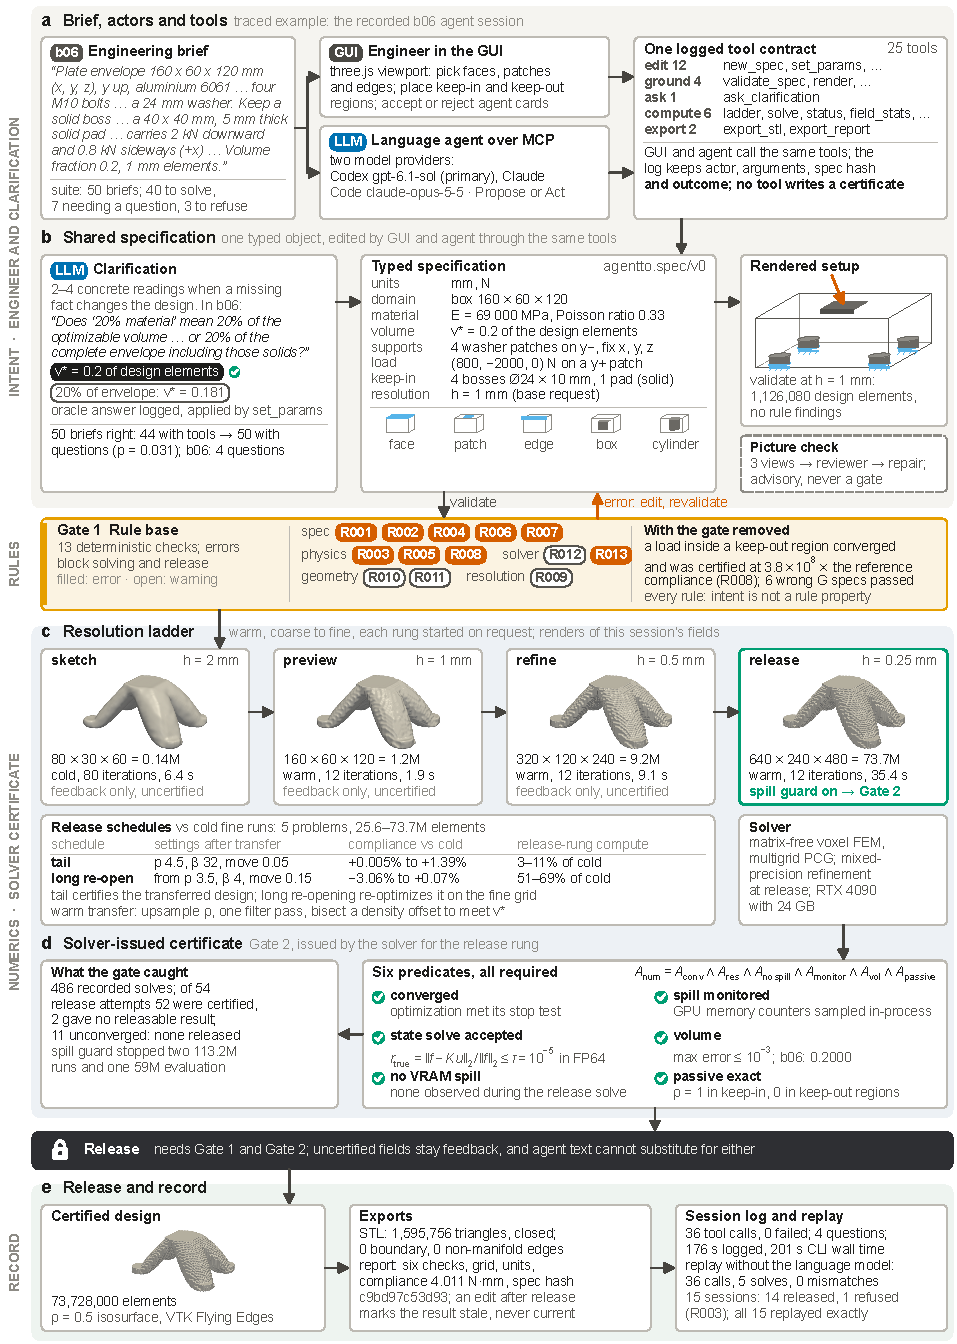
\includegraphics[width=156mm]{fig1_workflow.pdf}}
\caption{The AgenticTO workflow traced through one recorded agent session on the motor-mount brief b06, reproduced from
Figure~1 of the paper. The engineer and clarification settle intent, the rule gate admissibility and the solver
certificate numerical acceptance. Renders are $\rho=0.5$ isosurfaces of the saved fields; under the tail schedule the
fine rungs keep the transferred voxel steps.}
\label{fig:workflow}
\end{figure}

Figure~\ref{fig:workflow} follows one complete agent session through all of these pieces, from the brief to the
exported release. Chapter~\ref{ch:quickstart} repeats the same task by hand in the workspace.
